% Chemoattraction Model — Schematic (TikZ / LaTeX)
% ===================================================
% Stage: Publishing / Final paper figure
% Best for: LaTeX papers, journal submission, perfect math,
%           vector PDF output, consistent typography.
%
% Compile:
%   pdflatex schematic.tex
%
% Requires: TikZ, amsmath, amssymb
%           (all included in standard TeX Live / MikTeX)

\documentclass[tikz, border=12pt]{standalone}
\usepackage{tikz}
\usepackage{amsmath, amssymb}
\usetikzlibrary{
  arrows.meta,
  shapes.geometric,
  positioning,
  calc,
  backgrounds,
  fit,
  decorations.pathreplacing
}

% ── Reusable styles ───────────────────────────────────────────────────────────
\tikzset{
  % Cell shape
  cellnode/.style={
    ellipse, draw=#1!70!black, fill=#1!25, thick,
    minimum width=2.4cm, minimum height=1.9cm
  },
  % Generic rounded box
  roundbox/.style={
    rounded corners=7pt,
    draw=#1!70!black, fill=#1!18, thick,
    minimum width=4.0cm, minimum height=1.1cm,
    align=center, font=\small\bfseries
  },
  % Small annotation box
  annobox/.style={
    rounded corners=4pt,
    draw=#1!60!black, fill=#1!15,
    inner sep=4pt, align=center, font=\scriptsize
  },
  % Standard arrow
  myarrow/.style={
    ->, >=Stealth, thick, #1
  },
  % Dashed arrow
  dasharrow/.style={
    ->, >=Stealth, thick, dashed, #1
  },
}

\begin{document}
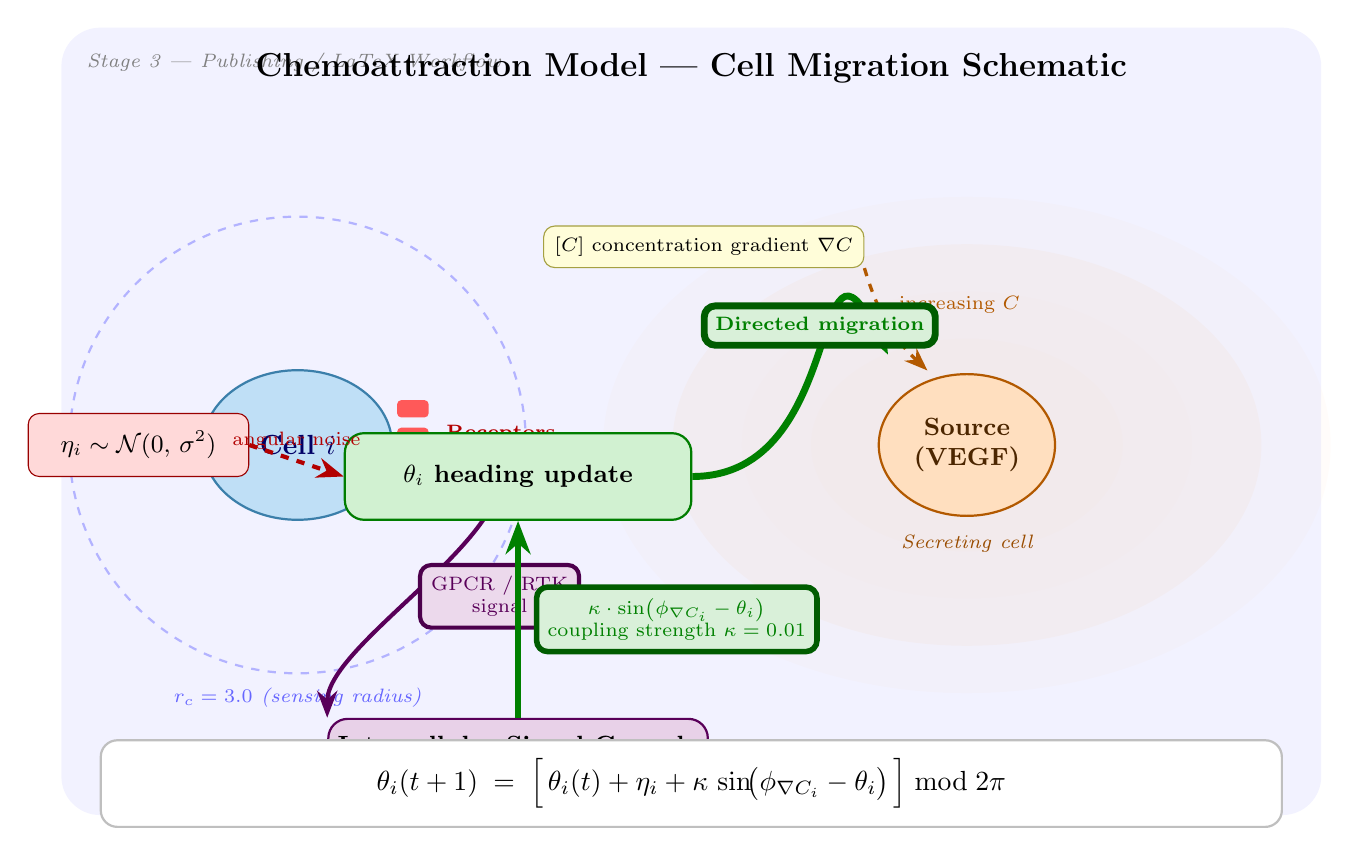
\begin{tikzpicture}

% ── Background panel ──────────────────────────────────────────────────────────
\fill[blue!5, rounded corners=14pt] (-2.5,-4.2) rectangle (13.5,5.8);

% Stage label
\node[font=\scriptsize\itshape, text=gray, anchor=north west] at (-2.3,5.6)
  {Stage 3 --- Publishing / LaTeX Workflow};

% Title
\node[font=\large\bfseries, anchor=north] at (5.5, 5.6)
  {Chemoattraction Model --- Cell Migration Schematic};

% ── Concentration gradient halo ───────────────────────────────────────────────
% Concentric ellipses fading outward from source at (9, 0.5)
\foreach \r/\op in {4.2/4, 3.4/7, 2.6/12, 1.8/18, 1.0/28}{
  \fill[orange!50, opacity=0.0\op]
    (9.0, 0.5) ellipse ({\r*1.1} and {\r*0.75});
}

% ── Source (secreting) cell ───────────────────────────────────────────────────
\node[cellnode=orange, minimum width=1.8cm, minimum height=1.8cm,
      font=\small\bfseries, align=center, text=orange!30!black]
  (source) at (9.0, 0.5)
  {Source\\(VEGF)};

\node[font=\scriptsize\itshape, text=orange!60!black,
      below=0.1cm of source] {Secreting cell};

% Gradient label with dashed arrow
\node[annobox=yellow, above left=1.6cm and 0.5cm of source]
  (gradlabel) {$[C]$ concentration gradient $\nabla C$};

\draw[dasharrow=orange!70!black, line width=1.2pt]
  (gradlabel.south east) to[bend right=15]
  node[midway, above right, font=\scriptsize, text=orange!70!black]
    {increasing $C$}
  ($(source.north west)+(0.3,0.3)$);

% ── Sensing cell i ────────────────────────────────────────────────────────────
\node[cellnode=cyan!80!blue, font=\normalsize\bfseries,
      text=blue!40!black]
  (cell) at (0.5, 0.5) {Cell $i$};

% Receptors (three small rectangles on right edge)
\foreach \dy in {0.35, 0.0, -0.35}{
  \fill[red!65, rounded corners=1.5pt]
    ($(cell.east)+(0.05,\dy)$) rectangle ++(0.40, 0.22);
}
\node[font=\scriptsize\bfseries, text=red!70!black,
      right=0.55cm of cell, align=left]
  (reclabel) {Receptors\\(VEGFR)};

% Sensing radius dashed ring
\draw[draw=blue!50, dashed, thick, opacity=0.55]
  (cell.center) circle (2.9cm);
\node[font=\scriptsize\itshape, text=blue!60,
      below=2.0cm of cell]
  {$r_c = 3.0$ (sensing radius)};

% ── Intracellular cascade ─────────────────────────────────────────────────────
\node[roundbox=violet, below=2.5cm of cell, xshift=2.8cm,
      minimum width=4.4cm]
  (cascade)
  {Intracellular Signal Cascade\\
   \normalfont\scriptsize PI3K / Rac1 / actin polarization};

% Arrow: receptor → cascade
\draw[myarrow=violet!70!black, line width=1.5pt]
  (reclabel.south)
    .. controls ++(0.0,-0.9) and ++(0.0, 0.9) ..
  (cascade.north west)
  node[midway, annobox=violet, right=0.05cm]
    {GPCR / RTK\\signal};

% ── Heading update box ────────────────────────────────────────────────────────
\node[roundbox=green!70!black, above=2.5cm of cascade, xshift=0cm,
      minimum width=4.4cm]
  (orient)
  {$\theta_i$ heading update};

% Arrow: cascade → heading update
\draw[myarrow=green!50!black, line width=2pt]
  (cascade.north) -- (orient.south)
  node[midway, annobox=green!60!black, right=0.1cm, xshift=0.1cm]
    {$\kappa \cdot \sin\!\left(\phi_{\nabla C_i} - \theta_i\right)$\\
     \normalfont\scriptsize coupling strength $\kappa = 0.01$};

% Arrow: directed migration toward source
\draw[myarrow=green!50!black, line width=2.5pt]
  (orient.east)
    .. controls ++(2.0, 0) and ++(-1.0, 2.0) ..
  ($(source.north west)+(-0.2, 0.5)$)
  node[midway, annobox=green!60!black, above=0.1cm]
    {\bfseries Directed migration};

% ── Angular noise ─────────────────────────────────────────────────────────────
\node[annobox=red, left=1.2cm of orient, yshift=0.4cm,
      minimum width=2.8cm, minimum height=0.8cm,
      font=\small]
  (noise)
  {$\eta_i \sim \mathcal{N}(0,\,\sigma^2)$};

\draw[dasharrow=red!70!black, line width=1.5pt]
  (noise.east) -- (orient.west)
  node[midway, above, font=\scriptsize, text=red!70!black]
    {angular noise};

% ── Equation footer ───────────────────────────────────────────────────────────
\node[draw=gray!50, fill=white, thick, rounded corners=6pt,
      font=\normalsize, align=center,
      minimum width=15.0cm, minimum height=1.1cm]
  at (5.5, -3.8)
  {$\theta_i(t+1) \;=\;
    \Bigl[\,\theta_i(t)
          + \eta_i
          + \kappa\,\sin\!\bigl(\phi_{\nabla C_i} - \theta_i\bigr)
    \,\Bigr] \bmod 2\pi$};

\end{tikzpicture}
\end{document}
